\subsubsection{Detector Support}

\fixme{This section is very detailed. We need to be more concise.}
The Detector Support System (DSS) provides the main structural support
for the single-phase detector.  The detector elements supported by the
DSS include the field cage endwalls, the \dwords{apa}, and
the \dwords{cpa} with top and bottom field cage panels.  The DSS is
supported by the cryostat outer steel structure through a series of
feedthrus which cross through the cryostat insulation and are anchored
with flanges on the cryostat roof. Inside the cryostat a series of
stainless steel I-beams are connected to the feedthrus and used to
support the detector. The DSS defines the location of the detector
inside the cryostat and it also defines how the detector elements move
as the detector is brought to \dword{lar} temperature. The design of the DSS
encompasses the overall structural design of the detector as only
after the elements are mounted to the DSS and are connected together
do they make a unified mechanical structure. The requirements of the
DSS are as follows:
%\begin{itemize}
%  \item[] {\bf DSS REQUIREMENTS}
%\end{itemize}
\begin{itemize}
 \setlength\itemsep{1mm}
\setlength{\parsep}{1mm}
\setlength{\itemsep}{-4mm}
% \small
\item Support the weight, both dry and wet [warm and cold?], of
  the detector (endwall, top/bottom FC, \dword{apa}, \dword{cpa})
\item Accommodate the roof movement [ROOF DEFORMATIONS NEED TO BE DEFINED]
\item Accommodate variation in the feedthrough locations and
  variation in the flange angles due to installation tolerances and
  loading on the warm structure.
\item Accommodate shrinkage of the detector and DSS from ambient
  temperature to \dword{lar} temperature.
\item Minimize the gaps that develop between \dwords{apa} during cool down to
  less than \SI{13}{mm}. [WHAT IS THE CORRECT VALUE?]  %A proposed  design uses beams that are 6.4m long, which support $\sim$3 \dwords{apa}.  This design results in no gap developing between the three \dwords{apa} on  the same beam but a 17~mm gap opening up between adjacent \dwords{apa} on  separate beams.  There will be a 17~mm gap between every 3$^{rd}$  and 4$^{th}$ \dword{apa}.
\item Accommodate installation of the detector. 
\item Define the position of the detector components relative to each other. [NEED TO DEFINE THIS TOLERANCE]
\item The \dword{cpa} to \dword{apa} centerline distance and tolerance envelope must be maintained at 3574$\pm y$~mm
\item The DSS is electrically connected to the cryostat ground
\item The \dword{apa}/\dword{cpa}/FC/endwall are electrically isolated from the DSS
\item The DSS penetrations must be purged with GAr to maintain a positive pressure in order to prevent contaminants from diffusing back into the liquid
\item The instrumentation cabling must not interfere with the DSS.
\item The DSS components must be able to be installed through the TCO
%\item A QA program is required
\item The DSS is to designed to meet AISC-360 and appropriate codes required by SURF
\item The DSS will be designed to meet seismic requirements 1 mile underground at SURF
\item All materials must be compatible for operation in ultrapure \dword{lar}
\item The DSS beams will be completely submerged in \dword{lar}
\item The DSS will ensure that detector components shall not be less than \SI{400}{mm} from the membrane flat surface
\item The DSS supports shall not interfere with the cryostat I-beam structures
\item The DSS shall be designed such that it supports the detector so that the lower ground plane is above the cryogenic piping and the top of the DSS beams are submerged in \dword{lar} while leaving a 4\% ullage at the top of the cryostat.
\item The DSS shall have infrastructure necessary to move the \dword{apa} and \dword{cpa}-FC assemblies from outside the cryostat through the TCO and to the correct position.
\end{itemize}

Figure~\ref{DSS} (left) shows the DSS structure; there are five rows
of supports for the alternating rows
of \dword{apa}-\dword{cpa}-\dword{apa}-\dword{cpa}-\dword{apa}.  The
DSS is connected to the warm structure at a flange that is mounted on
the outside of the cryostat.  Figure~\ref{DSS} (right) shows the
layout of these structural feedthroughs.  The DSS consists of pairs of
feedthroughs that support \SI{6.4}{m}-long S8x18.4 stainless steel I-beam
sections. The proposed design of the DSS has \num{10} I-beam segments per
row for a total of \num{50} I-beam segments. Each I-beam is suspended on
both ends by rods from feedthroughs that penetrate the roof.  In the
cold condition each beam will shrink which will cause gaps to form
between \dwords{apa} that are adjacent but supported on separate
beams.  \dwords{apa} that are supported on the same beam will not have
gaps develop because both the beam and \dwords{apa} are stainless
steel so they will shrink together.  Each beam is supported by a
nearly \SI{2}{m} long rod that allows the beam support to move as the beam
contracts.

\fixme{too much detail}
The feedthrough consists of a flange and $8 ^{''}$ OD structural tube
welded to it that extends through the cryostat insulation.  There is a
nominal \SI{10}{mm} gap between the OD of the tube and the ID of the
clearance tube in the cryostat.  The purpose of the $8 ^{''}$ tube is
to provide lateral support to the I-beams during installation.
Running down the center of the feedthrough is a 1� diameter rod that
is supported at a swivel washer at the flange and then supports the
I-beam at a clevis.  The gas seal is obtained by Conflat Flange and a
bellows that seals around the swivel washer.  The lateral position of
the rod can be adjusted to adjust the height of the DSS I-beams.
\begin{figure}[htbp]
\begin{center}
\begin{minipage}[c]{0.49\textwidth}
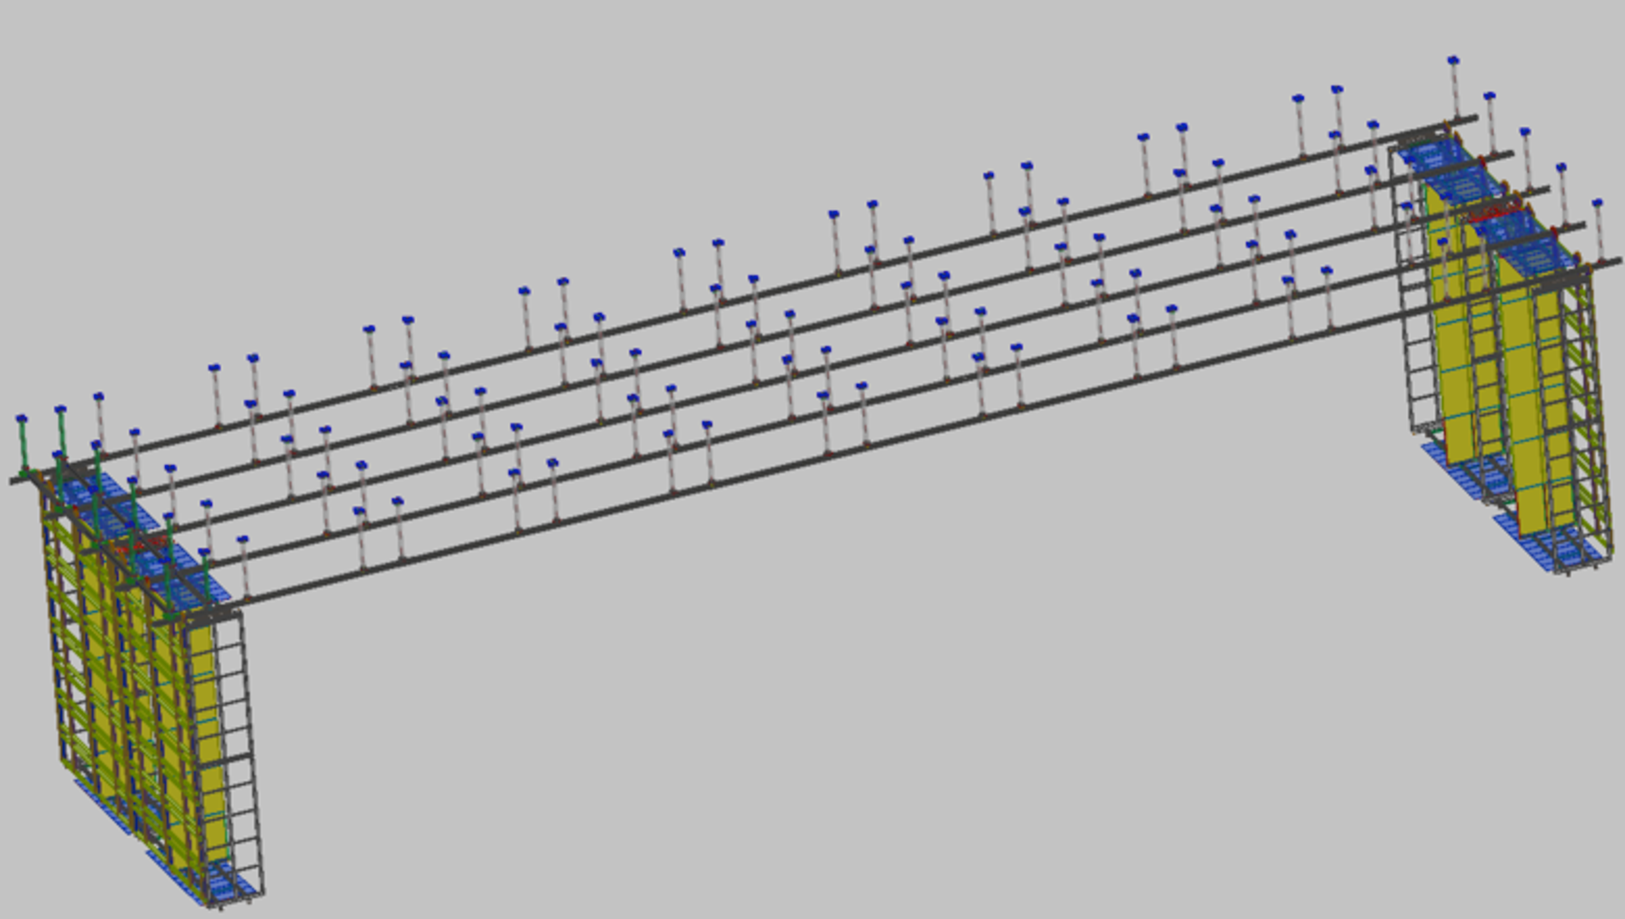
\includegraphics[width=\textwidth]{far-detector-single-phase/figures/DSS-1.pdf}
\end{minipage}
\begin{minipage}[c]{0.49\textwidth}
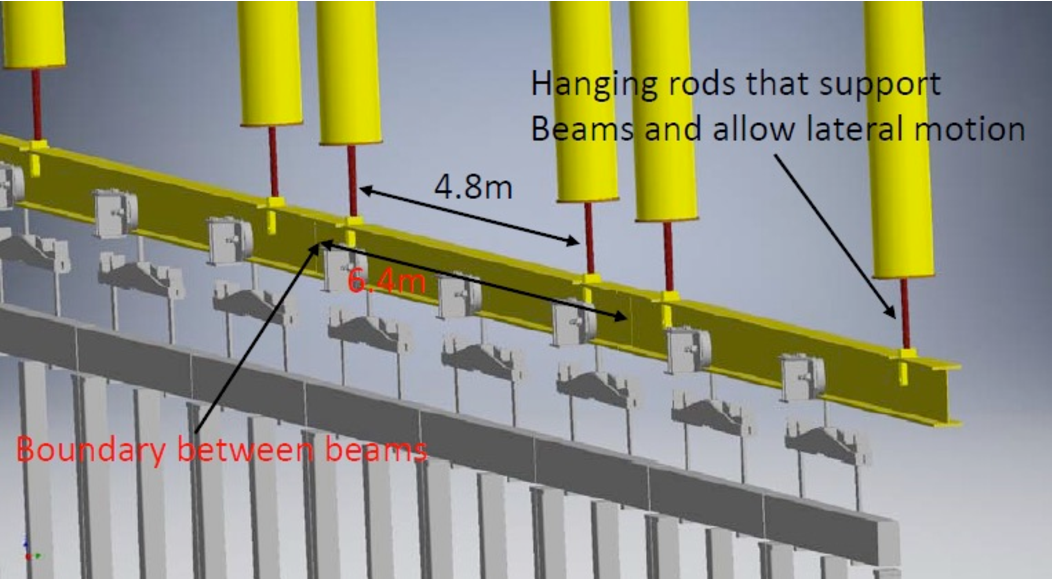
\includegraphics[width=\textwidth]{far-detector-single-phase/figures/DSS-2.pdf}
\end{minipage}
\caption{3-D model of the Detector Support System showing the entire structure on the left along with one row of \dword{apa} and \dword{cpa}/FC at each end. The right panel is a zoomed image showing the connections between the vertical supports and the horizontal I-beams.}
\label{DSS}
\end{center}
\end{figure}


Detector components will be installed using a shuttle beam system
illustrated in Fig.~\ref{shuttle}.  The last two columns of
feedthroughs (eastern most) will support temporary beams that run
north-south, perpendicular to the main DSS beams.  A shuttle beam
%shown in orange
will have trolleys mounted to it and will transverse
north-south until aligned with the required row of DSS beam.  The last
\dword{apa} or \dword{cpa} in a row is supported by the shuttle beam which is bolted
directly to the feedthroughs once it is in place.  As the last \dword{cpa} or
\dword{apa} in each row is installed the north-south beams are removed.

There will be a mechanical interlock system that prevents trolleys
from passing the end of the shuttle beam unless it is aligned with a
corresponding DSS beam.  The shuttle beam and each detector will be
moved using a motorized trolley.  A commercially available motorized
trolley will be modified as needed to meet the needs of the
installation.
\begin{figure}[htbp]
\begin{center}
\begin{minipage}[c]{0.49\textwidth}
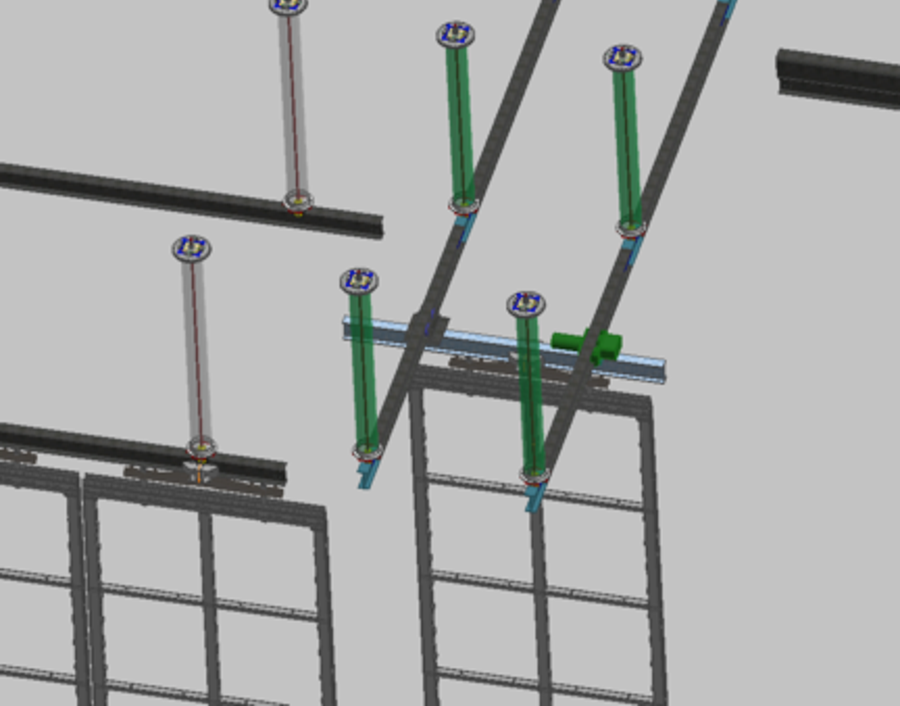
\includegraphics[width=\textwidth]{far-detector-single-phase/figures/Shuttle-1.pdf}
\end{minipage}
\begin{minipage}[c]{0.42\textwidth}
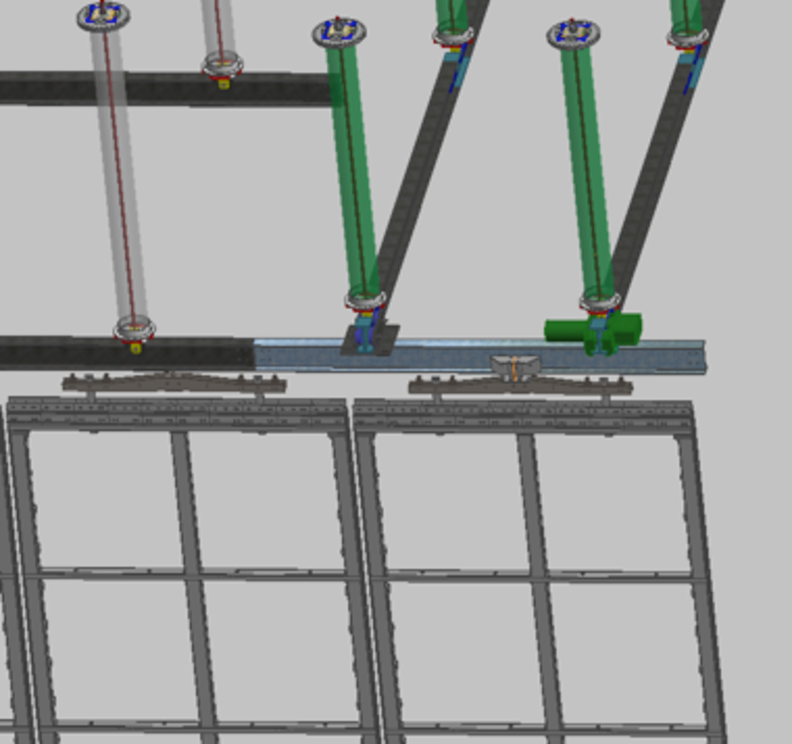
\includegraphics[width=\textwidth]{far-detector-single-phase/figures/shuttle-2.pdf}
\end{minipage}
\caption{3-D models of the shuttle beam end of the DSS. The figures show how an \dword{apa}
is translated into position using he North-South beams until it lines up with the correct
row of I-beams.}
\label{shuttle}
\end{center}
\end{figure}

The DSS installation begins with the placement and alignment of all
the feedthroughs onto the flanges that are mounted to the warm vessel.
There are \num{25} feedthroughs per row and five rows for a total of \num{125}
feedthroughs.  A fixture with a tooling ball will be attached to the
clevis of each feedthrough.  The $XY$ position in the horizontal plane
and the vertical $Z$ position of this tooling ball will be defined.  A
survey will be performed to determine the location of each tooling
ball center and $XY$ and $Z$ adjustments will be made to get the tooling
ball centers to within $\pm$\SI{3}{mm}.  The \SI{6.4}{m} long I-beams will then be
raised and pinned to the clevis.  Each beam weights roughly 350~lbs.
A lifting tripod will be placed over each of the feedthroughs
supporting a beam and a $1/4 ^{''}$ cable will be fed through the top
flange of the feedthrough down the \SI{14}{m} to the cryostat floor where it
will be attached to the I-beam.  The winches on each tripod will raise
the beam in unison in order to get it to the correct height to be
pinned to the feedthrough clevis.  Once the beams are mounted a final
survey of the beams will occur to ensure they are located and aligned
to each other properly.

A mock up of the shuttle system will be constructed to test the
mechanical interlock and drive systems for the shuttle beam
for each detector.  Tests will be conducted to evaluate the level of
misalignment between beams that can be tolerated and the amount of
positional control that can be achieved with the motorized trolley. It
is expected this will be finished prior to the TDR. At the time of the
TDR a larger prototype installation at Ash River will be under
construction. This prototype will use full scale elements and will be
used to develop the installation procedures and to also test the
detector installation process.

\fixme{concluding paragraph?}
